
\chapter{سند موارد کاربرد}


\section{توصیف کنش‌گرها}


\begin{table}[H]
	\centering
	\begin{tabular}{|p{3cm}|p{8cm}|}
		\hline
		
		
		کنشگر	& توصیف  \\
		\hline
		
		نیروی انسانی سازمان &
		
		نیروی انسانی سازمان، هر فردی است که در سازمان استخدام شده است و دارای حساب کاربری در سیستم برنامه‌ریزی است.\\
		
		\hline
		
	\end{tabular}
\end{table}

\begin{table}[H]
	\centering
	\begin{tabular}{|p{3cm}|p{8cm}|}
		\hline
		
		
		کنشگر	& توصیف  \\
		\hline
		مدیر پروژه &
		
		مدیر پروژه یک نیروی انسانی سازمان است که سیستم‌ها، ماژول‌های سیستم و افرادی را که در این پروژه مشارکت دارند به همراه کاری (تسکی) که انجام می‌دهند مشخص می‌کند، منابع را تخصیص می‌دهد، زمانبندی‌ها را انجام می‌دهد و همچنین سطوح دسترسی افراد درگیر در پروژه را مشخص می‌کند.
		\\
		\hline
		
	\end{tabular}
\end{table}


\begin{table}[H]
	\centering
	\begin{tabular}{|p{3cm}|p{8cm}|}
		\hline
		
		
		کنشگر	& توصیف  \\
		\hline
		زمان &
		
		عملیاتی که در سیستم برنامه‌ریزی در زمان خاص و مشخص انجام می‌شوند، تحت فرمان این کنشگر هستند.
		\\
		\hline
		
	\end{tabular}
\end{table}

\begin{table}[H]
	\centering
	\begin{tabular}{|p{3cm}|p{8cm}|}
		\hline
		
		
		کنشگر	& توصیف  \\
		\hline
		کاربر &
		
	هر فردی که با سیستم  برنامه‌ریزی تعامل دارد، یک کاربر محسوب می‌شود.
		\\
		\hline
		
	\end{tabular}
\end{table}


\begin{table}[H]
	\centering
	\begin{tabular}{|p{3cm}|p{8cm}|}
		\hline
		
		
		کنشگر	& توصیف  \\
		\hline
		مدیر &
		
		نیروی انسانی سازمان است که به نوعی در مقام مدیریت شرکت باشد. این افراد تمامی امکاناتی را که یک کارمند معمولی  دارد، دارا است. علاوه بر این، تعدادی از عملیات مخصوص این افراد است که به نظارت و مدیریت سیستم برنامه‌ریزی باز می‌گردد.
		\\
		\hline
		
	\end{tabular}
\end{table}

\newpage
\section{نمودارهای موارد کاربرد}

\subsection{زیرسیستم تولید و نگهداری}
\begin{figure}[H]
	\centering
	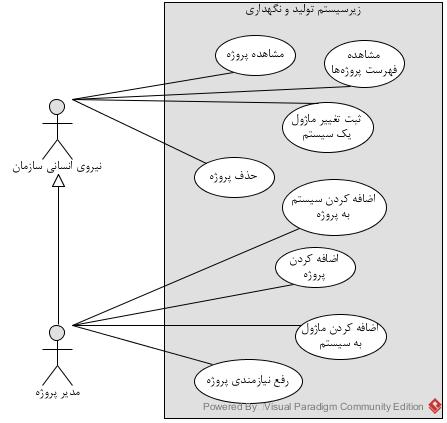
\includegraphics[scale=0.8]{img/usecase/tolid}
	\caption{زیرسیستم تولید و نگهداری}
\end{figure}

\subsection{زیرسیستم توزیع}
\begin{figure}[H]
	\centering
	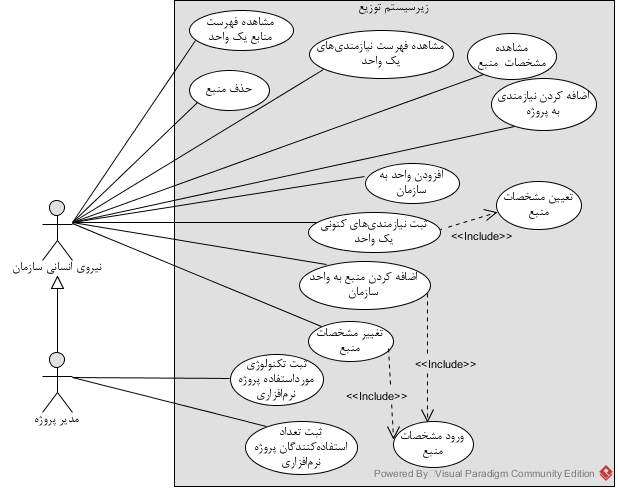
\includegraphics[scale=0.8]{img/usecase/tozi}
	\caption{زیرسیستم توزیع}
\end{figure}

\subsection{زیرسیستم گزارش‌گیری}
\begin{figure}[H]
	\centering
	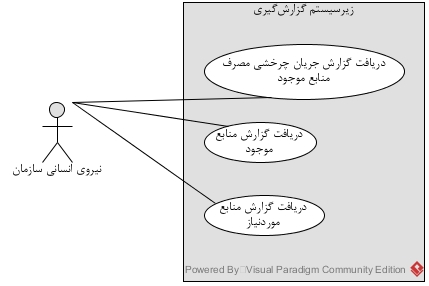
\includegraphics[scale=1]{img/usecase/report}
	\caption{زیرسیستم گزارش‌گیری}
\end{figure}

\subsection{زیرسیستم پیش‌بینی}
\begin{figure}[H]
	\centering
	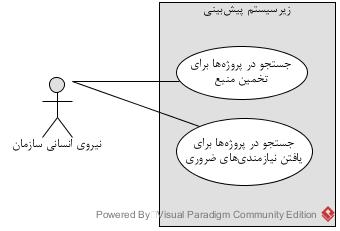
\includegraphics[scale=1]{img/usecase/est}
	\caption{زیرسیستم پیش‌بینی}
\end{figure}

\subsection{زیرسیستم کاربری}
\begin{figure}[H]
	\centering
	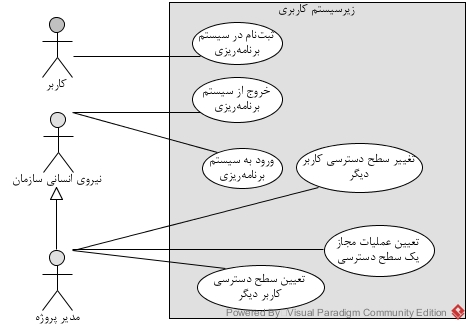
\includegraphics[scale=0.9]{img/usecase/user}
	\caption{زیرسیستم کاربری}
\end{figure}

\subsection{زیرسیستم پشتیبانی}
\begin{figure}[H]
	\centering
	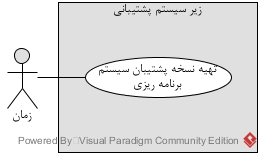
\includegraphics[scale=1]{img/usecase/support}
	\caption{زیرسیستم پشتیبانی}
\end{figure}

\newpage
\section{توصیف موارد کاربرد}
\subsection{زیرسیستم تولید و نگهداری}

\begin{table}[H]
	\centering
	\begin{tabular}{|p{3cm}|p{10cm}|}
		\hline
		
		
		مورد کاربرد	& اضافه کردن پروژه  \\
		\hline
		
		شناسه & 
		\stepcounter{usecase_ID}
		
		\arabic{usecase_ID} \\
		
		\hline
		
		توضیح مختصر & مدیر پروژه، یک پروژه به مجموعه پروژه‌های سازمان اضافه می‌کند و اطلاعات مربوط به آن را وارد سیستم برنامه‌ریزی می‌کند. \\
		\hline
		
		کنشگر(های) اولیه & مدیر پروژه \\
		\hline
		
		کنشگر(های) ثانویه&  \\
		\hline
		
		پیش‌نیازها &
		مدیر پروژه در سیستم برنامه‌ریزی وارد شده است.\\
		\hline
		
		
		روند اصلی &
		\begin{enumerate}[topsep=0cm,leftmargin=0.5cm]
			\item مدیر پروژه درخواست اضافه کردن پروژه را می‌دهد.
			\item سیستم برنامه‌ریزی نام پروژه را درخواست می‌کند.
			\item مدیر پروژه نام پروژه را وارد می‌کند. 
			\item سیستم برنامه‌ریزی نام واحد(های) درگیر در پروژه را درخواست می‌کند. 
			\item مدیر پروژه واحد(های) درگیر در پروژه را اعلام می‌کند. 
			\item  مدیر پروژه اطلاعات وارد شده را تایید می‌کند. 
			\item سیستم برنامه‌ریزی پروژه جدید را ثبت می‌کند.
		\end{enumerate} \\
		
		\hline
		
		پس‌نیازها &
		پروژه‌ی موردنظر به سیستم برنامه‌ریزی اضافه می‌شود. \\
		\hline
		
		روند جایگزین & انصراف \\
		\hline
		
	\end{tabular}
\end{table}


\begin{table}[H]
	\centering
	\begin{tabular}{|p{3cm}|p{10cm}|}
		\hline
		
		
		مورد کاربرد	& روند جایگزین "اضافه کردن پروژه": انصراف  \\
		\hline
		
		شناسه & 
		\stepcounter{usecase_AF}
		
		\arabic{usecase_ID}.\arabic{usecase_AF} \\
		
		\hline
		
		توضیح مختصر & مدیر پروژه از اضافه کردن پروژه انصراف می‌دهد. \\
		\hline
		
		کنشگر(های) اولیه& مدیر پروژه \\
		\hline
		
		کنشگر(های) ثانویه&  \\
		\hline
		
		پیش‌نیازها &
		مدیر پروژه اضافه کردن پروژه را انتخاب کرده است.\\
		\hline
		
		
		روند اصلی &
		\begin{enumerate}[topsep=0cm,leftmargin=0.5cm]
			\item روند جایگزین از اتمام مرحله 1 و یا مراحل بعدی می‌تواند شروع شود.
			\item مدیر پروژه از ادامه مراحل و اضافه کردن پروژه منصرف می‌شود. 
			\item مدیر پروژه انصراف را انتخاب می‌کند. 
		\end{enumerate} \\
		\hline
		
		پس‌نیازها &
		ندارد. \\
		\hline
		
		روند جایگزین & ندارد. \\
		\hline
		
	\end{tabular}
\end{table}

\begin{table}[H]
	\centering
	\begin{tabular}{|p{3cm}|p{10cm}|}
		\hline
		
		مورد کاربرد & مشاهده پروژه  \\
		\hline
		
		شناسه & 
		\stepcounter{usecase_ID}
		
		\arabic{usecase_ID} \\
		\hline
		
		توضیح مختصر & نیروی انسانی سازمان اطلاعات مربوط به یک پروژه را مشاهده می‌کند. \\
		\hline
		
		کنشگر(های) اولیه & نیروی انسانی سازمانی \\
		\hline
		
		کنشگر(های) ثانویه &  \\
		\hline
		
		پیش‌نیازها & نیروی انسانی سازمان وارد سیستم برنامه‌ریزی شده است. \\
		\hline
		
		
		روند اصلی &
		\begin{enumerate}[topsep=0cm,leftmargin=0.5cm]
			
			\item نیروی انسانی سازمان درخواست مشاهده‌ی پروژه را می‌دهد. 
			\item سیستم برنامه‌ریزی نام پروژه را درخواست می‌کند. 
			\item نیروی انسانی سازمان نام پروژه را وارد می‌کند. 
			\item تا زمانی که نام پروژه صحیح نیست: 
			\begin{enumerate}[topsep=0cm,leftmargin=0.5cm]
				\item سیستم برنامه‌ریزی نام پروژه را درخواست می‌کند. 
				\item نیروی انسانی سازمان نام پروژه را وارد می‌کند.
			\end{enumerate}
			\item سیستم برنامه‌ریزی فهرست سیستم‌ها، ماژول‌ها و منابع پروژه را نمایش می‌دهد.
		\end{enumerate} \\
		\hline
		
		
		پس‌نیازها & ندارد. \\
		\hline
		
		روند جایگزین & انصراف \\
		\hline
		
	\end{tabular}
\end{table}


\begin{table}[H]
	\centering
	\begin{tabular}{|p{3cm}|p{10cm}|}
		\hline
		
		مورد کاربرد & مشاهده فهرست پروژه‌ها  \\
		\hline
		
		شناسه & 
		\stepcounter{usecase_ID}
		
		\arabic{usecase_ID} \\
		\hline
		
		توضیح مختصر & نیروی انسانی سازمان فهرست پروژه‌های سازمان را مشاهده می‌کند. \\
		\hline
		
		کنشگر(های) اولیه & نیروی انسانی سازمان \\
		\hline
		
		کنشگر(های) ثانویه &  \\
		\hline
		
		پیش‌نیازها & نیروی انسانی سازمان وارد سیستم برنامه‌ریزی شده است. \\
		\hline
		
		
		روند اصلی &
		\begin{enumerate}[topsep=0cm,leftmargin=0.5cm]
			
			\item نیروی انسانی سازمان درخواست مشاهده فهرست پروژه‌ها را می‌دهد.
			\item سیستم برنامه‌ریزی فهرست پروژه‌های سازمان را نمایش می‌دهد.
		\end{enumerate} \\
		
		\hline
		
		پس‌نیازها & فهرست پروژه‌های سازمان نمایش داده می‌شود. \\
		\hline
		
		روند جایگزین &  \\
		\hline
		
	\end{tabular}
\end{table}

\begin{itemize}
	\item این روند جایگزین به طور مشابه برای تمامی موارد کاربردی که در آن انصراف به عنوان روند جایگزین ذکر شده است، صدق می‌کند. به همین علت از تکرار آن خودداری می‌کنیم.
\end{itemize}

\begin{table}[H]
	\centering
	\begin{tabular}{|p{3cm}|p{10cm}|}
		\hline
		
		
		مورد کاربرد	& اضافه کردن سیستم به پروژه  \\
		\hline
		
		شناسه & 
		\stepcounter{usecase_ID}
		
		\arabic{usecase_ID} \\
		
		\hline
		
		توضیح مختصر & مدیر پروژه، یک پروژه را از بین مجموعه پروژه‌های سازمان انتحاب می‌کند و یک سیستم به مجموعه سیستم‌های آن پروژه اضافه می‌کند و اطلاعات مربوط به آن را وارد سیستم برنامه‌ریزی می‌کند. \\
		\hline
		
		کنشگر(های) اولیه & مدیر پروژه \\
		\hline
		
		کنشگر(های) ثانویه&  \\
		\hline
		
		پیش‌نیازها &
		مدیر پروژه در سیستم برنامه‌ریزی وارد شده است.\\
		\hline
		
		
		روند اصلی &
		\begin{enumerate}[topsep=0cm,leftmargin=0.5cm]
			\item مدیر پروژه درخواست اضافه کردن سیستم را می‌دهد.
			\item  سیستم برنامه‌ریزی نام پروژه را درخواست می‌کند.
			\item مدیر پروژه نام پروژه را وارد می‌کند.
			\item تا زمانی که نام پروژه صحیح نیست:
			\begin{enumerate}[topsep=0cm, leftmargin=0.5cm]
				\item سیستم برنامه‌ریزی نام پروژه را درخواست می‌کند.
				\item مدیر پروژه نام پروژه‌ مورد نظر را وارد می‌کند.
			\end{enumerate}
			\item  سیستم برنامه‌ریزی، نام سیستم را درخواست می‌کند.
			\item مدیر پروژه نام سیستم را وارد می‌کند.
			\item  مدیر پروژه اطلاعات وارد شده را تایید می‌کند.
			\item سیستم برنامه‌ریزی، سیستم جدید را ثبت می‌کند.
		\end{enumerate} \\
		
		\hline
		
		پس‌نیازها &
		سیستم مورد نظر به مجموعه سیستم‌های پروژه‌ی انتخاب شده در سیستم برنامه‌ریزی اضافه می‌شود. \\
		\hline
		
		روند جایگزین & انصراف \\
		\hline
		
	\end{tabular}
\end{table}

\begin{table}[H]
	\centering
	\begin{tabular}{|p{3cm}|p{10cm}|}
		\hline
		
		
		مورد کاربرد	& اضافه کردن ماژول به سیستم \\
		\hline
		
		شناسه & 
		\stepcounter{usecase_ID}
		
		\arabic{usecase_ID} \\
		
		\hline
		
		توضیح مختصر & مدیر پروژه، یک پروژه از بین مجموعه پروژه‌های سازمان و یک سیستم آن پروژه را انتخاب کرده و یک ماژول به آن اضافه می‌کند. \\
		\hline
		
		کنشگر(های) اولیه& مدیر پروژه \\
		\hline
		
		کنشگر(های) ثانویه&  \\
		\hline
		
		پیش‌نیازها &
		مدیر پروژه در سیستم برنامه‌ریزی وارد شده است.\\
		\hline
		
		
		روند اصلی &
		\begin{enumerate}[topsep=0cm,leftmargin=0.5cm]
			\item  مدیر پروژه درخواست اضافه کردن ماژول را می‌دهد.
			\item سیستم برنامه‌ریزی نام پروژه را درخواست می‌کند.
			\item مدیر پروژه نام پروژه مورد نظر را وارد می‌کند. 
			\item تا زمانی که نام پروژه صحیح نیست:
			\begin{enumerate}[topsep=0cm,leftmargin=0.5cm]
				\item سیستم برنامه‌ریزی نام پروژه را درخواست می‌کند.
				\item مدیر پروژه نام پروژه‌ مورد نظر را وارد می‌کند.
			\end{enumerate}
			\item  سیستم برنامه‌ریزی نام سیستم را درخواست می‌کند.
			\item  مدیر پروژه نام سیستم مورد نظر را وارد می‌کند. 
			\item  تا زمانی که نام سیستم صحیح نیست:
			\begin{enumerate}[topsep=0cm,leftmargin=0.5cm]
				\item سیستم برنامه‌ریزی نام سیستم را درخواست می‌کند.
				\item مدیر پروژه نام سیستم مورد نظر را وارد می‌کند.
			\end{enumerate}
			\item  سیستم برنامه‌ریزی نام ماژول و ایجادکننده (یا ایجادکنندگان)  را درخواست می‌کند.
			\item مدیر پروژه نام ماژول و ایجادکننده (یا ایجادکنندگان) را وارد می‌کند.
			\item تا زمانی که مدیر پروژه درخواست افزودن منبع را به سیستم برنامه‌ریزی می‌دهد:
			\begin{enumerate}[topsep=0cm,leftmargin=0.5cm]
				\item سیستم برنامه‌ریزی فهرست تمام منابع موجود در واحدهای درگیر در آن پروژه را ارائه می‌دهد.
				\item include (انتخاب منبع)
			\end{enumerate}
			\item سیستم برنامه‌ریزی ماژول مورد نظر را به ماژول‌های سیستم اضافه می‌کند.
		\end{enumerate} \\
		\hline
		
		پس‌نیازها &
		ماژول موردنظر به سیستم اضافه می‌شود. \\
		& منابع درخواستی مدیر پروژه از منابع موجود در واحدهای درگیر کم می‌شود.\\
		
		\hline
		
		روند جایگزین
		& انصراف \\
		\hline
		
	\end{tabular}
\end{table}


\begin{table}[H]
	\centering
	\begin{tabular}{|p{3cm}|p{10cm}|}
		\hline
		
		
		مورد کاربرد	& انتخاب منبع  \\
		\hline
		
		شناسه & 
		\stepcounter{usecase_ID}
		
		\arabic{usecase_ID} \\
		
		\hline
		
		توضیح مختصر & مدیر پروژه با توجه به فهرست منابع موجود، منبع مورد نظر را انتخاب می‌کند و براساس نوع آن، اطلاعات خواسته شده را وارد می‌کند. \\
		\hline
		
		کنشگر(های) اولیه& - \\
		\hline
		
		کنشگر(های) ثانویه&  \\
		\hline
		
		پیش‌نیازها &
		مدیر پروژه در سیستم برنامه‌ریزی وارد شده است.\\
		& فهرست منابع، به مدیر پروژه ارائه شده است. \\
		\hline
		
		
		روند اصلی &
		\begin{enumerate}[topsep=0cm,leftmargin=0.5cm]
			\item  مدیر پروژه یک منبع را انتخاب می‌کند.
			\item اگر نوع منبع انتخابی منبع مالی نقدی باشد:
			\item تا زمانی که مبلغ وارد شده توسط مدیر پروژه بیشتر از میزان موجود است:
			\begin{enumerate}[topsep=0cm,leftmargin=0.5cm]
				\item سیستم برنامه‌ریزی مبلغ مورد نیاز را درخواست می‌کند.
				\item مدیر پروژه مبلغ مورد نیاز را وارد می‌کند.
			\end{enumerate}
			\item در غیر اینصورت، اگر نوع منبع انتخابی منبع فیزیکی باشد:
			\begin{enumerate}[topsep=0cm,leftmargin=0.5cm]
				\item تا زمانی که تعداد وارد شده توسط مدیر پروژه بیشتر از تعداد موجود است:
				\begin{enumerate}[topsep=0cm,leftmargin=0.5cm]
					\item سیستم برنامه‌ریزی تعداد مورد نیاز را درخواست می‌کند.
					\item مدیر پروژه تعداد مورد نیاز را وارد می‌کند.
				\end{enumerate}
			\end{enumerate}
			\item مدیر پروژه اطلاعات وارد شده را تایید می‌کند.
		\end{enumerate}\\
		\hline
		
		پس‌نیازها &
		ندارد. \\
		
		\hline
		
		روند جایگزین
		& انصراف \\
		\hline
		
	\end{tabular}
\end{table}





\begin{table}[H]
	\centering
	\begin{tabular}{|p{3cm}|p{10cm}|}
		\hline
		
		
		مورد کاربرد	& تخصیص منبع به پروژه  \\
		\hline
		
		شناسه & 
		\stepcounter{usecase_ID}
		
		\arabic{usecase_ID} \\
		
		\hline
		
		توضیح مختصر & مدیر پروژه یک پروژه را از بین مجموعه پروژه‌های سازمان انتخاب کرده و از بین منابع واحد‌های درگیر منبعی را به پروژه اضافه می‌کند. \\
		\hline
		
		کنشگر(های) اولیه & مدیر پروژه \\
		\hline
		
		کنشگر(های) ثانویه&  \\
		\hline
		
		پیش‌نیازها &
		مدیر پروژه در سیستم برنامه‌ریزی وارد شده است.\\
		\hline
		
		
		روند اصلی &
		\begin{enumerate}[topsep=0cm,leftmargin=0.5cm]
			\item مدیر پروژه درخواست اضافه کردن منبع به پروژه را می‌دهد.
			\item  سیستم برنامه‌ریزی، نام پروژه را درخواست می‌کند.
			\item مدیر پروژه نام پروژه‌ مورد نظر را وارد می‌کند.
			\item تا زمانی که نام پروژه صحیح نیست:
			\begin{enumerate}[topsep=0cm,leftmargin=0.5cm]
				\item سیستم برنامه‌ریزی، نام پروژه را درخواست می‌کند.
				\item مدیر پروژه نام پروژه‌ مورد نظر را وارد می‌کند.
			\end{enumerate}
			\item سیستم برنامه‌ریزی فهرست تمام منابع موجود در واحدهای درگیر در آن پروژه را ارائه می‌دهد.
			\item include (انتخاب منبع)
			\item  سیستم برنامه‌ریزی فرایندی را که منبع برای آن نیاز است درخواست می‌کند.
			\item  مدیر پروژه نام فرایندی که منبع برای آن نیاز است را وارد می‌کند.
			\item سیستم برنامه‌ریزی ضرورت یا عدم ضرورت منبع را برای پروژه درخواست می‌کند.
			\item مدیر پروژه، ضرورت یا عدم ضرورت منبع را برای پروژه وارد می‌کند.
			\item مدیر پروژه اطلاعات وارد شده را تایید می‌کند.
			\item سیستم برنامه‌ریزی منبع جدید را به منابع پروژه اضافه می‌کند.
			
		\end{enumerate} \\
		\hline
		
		پس‌نیازها &
		منبع درخواستی به منابع پروژه اضافه می‌شود. \\
		& منبع درخواستی مدیر پروژه از منابع موجود در واحدهای درگیر کم می‌شود.\\
		
		\hline
		
		روند جایگزین
		& انصراف \\
		\hline
		
	\end{tabular}
\end{table}



\begin{table}[H]
	\centering
	\begin{tabular}{|p{3cm}|p{10cm}|}
		\hline
		
		
		مورد کاربرد	& ثبت تغییر ماژول یک سیستم  \\
		\hline
		
		شناسه & 
		\stepcounter{usecase_ID}
		
		\arabic{usecase_ID} \\
		
		\hline
		
		توضیح مختصر & نیروی انسانی سازمان یک پروژه از بین مجموعه پروژه‌های سازمان، یک سیستم آن و یک ماژول آن سیستم را انتخاب کرده و تغییردهنده (تغییردهندگان)، نوع تغییر، مدت زمانی که صرف تغییر شده و منابع استفاده شده برای تغییر آن ماژول را ثبت می‌کند. \\
		\hline
		
		کنشگر(های) اولیه & نیروی انسانی سازمان \\
		\hline
		
		کنشگر(های) ثانویه&  \\
		\hline
		
		پیش‌نیازها &
		نیروی انسانی سازمان در سیستم برنامه‌ریزی وارد شده است.\\
		& نیروی انسانی سازمان مجاز به تغییر ماژول پروژه است. \\
		\hline
		
		
		روند اصلی &
		\begin{enumerate}[topsep=0cm,leftmargin=0.5cm]
			\item نیروی انسانی سازمان درخواست  ثبت تغییر انجام شده روی ماژول یک پروژه را می‌دهد.
			\item سیستم برنامه‌ریزی نام پروژه، نام سیستم و نام ماژول تغییر یافته را درخواست می‌کند.
			\item نیروی انسانی سازمان نام پروژه، نام سیستم و نام ماژول موردنظر را وارد می‌کند.
			\item تا زمانی که پروژه یا سیستم یا ماژول مورد نظر موجود نیست:
			\begin{enumerate}[topsep=0cm,leftmargin=0.5cm]
				\item سیستم برنامه‌ریزی سازمان نام پروژه، نام سیستم و نام ماژول تغییر یافته را درخواست می‌کند.
				\item نیروی انسانی سازمان نام پروژه‌، نام سیستم و نام ماژول موردنظر را وارد می‌کند. 
			\end{enumerate}
			\item سیستم برنامه‌ریزی نوع تغییر اعمال شده، مدت زمان اعمال تغییرات، نام تغییردهنده (تغییر دهندگان) و منابع  مصرف شده برای اعمال تغییرات را درخواست می‌کند.
			\item نیروی انسانی سازمان نوع تغییر اعمال شده، مدت زمان اعمال تغییرات، نام تغییردهنده (تغییر دهندگان)، منابع  مصرف شده برای اعمال تغییرات را وارد می‌کند.
			\item نیروی انسانی سازمان اطلاعات وارد شده را تایید می‌کند.
			\item سیستم برنامه‌ریزی تغییرات وارد شده را اعمال می‌کند. 
		\end{enumerate}\\
		
		\hline
		
		پس‌نیازها &
		تغییرات اعمال شده روی ماژول در سیستم برنامه‌ریزی ثبت می‌شود. \\
		
		\hline
		
		روند جایگزین
		& انصراف \\
		\hline
		
	\end{tabular}
\end{table}

\subsection{زیرسیستم توزیع}

\begin{table}[H]
	\centering
	\begin{tabular}{|p{3cm}|p{10cm}|}
		\hline
		
		مورد کاربرد	& اضافه کردن منبع به واحد سازمان  \\
		\hline
		
		شناسه & 
		\stepcounter{usecase_ID}
		
		\arabic{usecase_ID} \\
		
		\hline
		
		توضیح مختصر & نیروی انسانی سازمان یک واحد از سازمان را انتخاب کرده و منبع مورد نظر را به منابع آن واحد از سازمان اضافه می‌کند. \\
		\hline
		
		کنشگر(های) اولیه& نیروی انسانی سازمان \\
		\hline
		
		کنشگر(های) ثانویه&  \\
		\hline
		
		پیش‌نیازها &
		نیروی انسانی سازمان در سیستم برنامه‌ریزی وارد شده است.\\
		& نیروی انسانی سازمان مجاز به اضافه کردن منبع به واحد است. \\
		\hline
		
		
		روند اصلی &
		\begin{enumerate}[topsep=0cm,leftmargin=0.5cm]
			\item نیروی انسانی سازمان درخواست اضافه کردن منبع به واحد سازمان را می‌دهد.
			\item سیستم برنامه‌ریزی نام واحد را درخواست می‌کند.
			\item نیروی انسانی سازمان نام واحد مورد نظر را وارد می‌کند.
			\item تا زمانی که نام واحد وارد شده صحیح نیست:
			\begin{enumerate}[topsep=0cm,leftmargin=0.5cm]
				\item سیستم برنامه‌ریزی نام واحد را درخواست می‌کند.
				\item نیروی انسانی سازمان نام واحد مورد نظر را وارد می‌کند.
			\end{enumerate}
			\item سیستم برنامه‌ریزی نوع منبع را درخواست می‌کند.
			\item نیروی انسانی سازمان نوع منبع مورد نظر را وارد می‌کند.
			\item include (ورود مشخصات منبع)
			\item سیستم برنامه‌ریزی منبع جدید را به منابع واحد اضافه می‌کند
		\end{enumerate} \\
		
		\hline
		
		پس‌نیازها &
		منبع موردنظر به منابع واحد اضافه می‌شود. \\
		
		\hline
		روند جایگزین
		& انصراف \\
		\hline
		
	\end{tabular}
\end{table}


\begin{table}[H]
	\centering
	\begin{tabular}{|p{3cm}|p{11cm}|}
		\hline
		
		مورد کاربرد & ورود مشخصات منبع  \\
		\hline
		
		شناسه & 
		\stepcounter{usecase_ID}
		
		\arabic{usecase_ID} \\
		
		\hline
		
		توضیح مختصر & نیروی انسانی سازمان نوع منبع را انتخاب کرده و مشخصات منبع مورد نظر را وارد می‌کند. \\
		\hline
		
		کنشگر(های) اولیه& - \\
		\hline
		
		کنشگر(های) ثانویه&  \\
		\hline
		
		پیش‌نیازها &
		نیروی انسانی سازمان در سیستم برنامه‌ریزی وارد شده است.\\
		& نیروی انسانی سازمان نوع منبع را مشخص کرده است و درخواست وارد کردن مشخصات منبع را داده است. \\
		\hline
		
		
		روند اصلی &
		\begin{enumerate}[topsep=0cm,leftmargin=0.5cm]
			\item نیروی انسانی سازمان درخواست ورود مشخصات منبع را می‌دهد.
			\item اگر نوع منبع انتخابی منبع مالی باشد:
			\begin{enumerate}[topsep=0cm,leftmargin=0.5cm]
				\item سیستم برنامه‌ریزی نوع منبع مالی (نقدی یا غیرنقدی)، مبلغ منبع مالی و محلی که در آن جا وجود دارد را درخواست می‌کند.
				\item نیروی انسانی سازمان نوع منبع مالی (نقدی یا غیرنقدی)، مبلغ منبع مالی و محلی که در آن جا وجود دارد را وارد می‌کند.
			\end{enumerate}
			\item در غیر اینصورت اگر نوع منبع انتخابی منبع انسانی باشد:
			\begin{enumerate}[topsep=0cm,leftmargin=0.5cm]
				\item سیستم برنامه‌ریزی نام و نام خانوادگی، پست شغلی در سازمان، کد پرسنلی، تخصص‌های آن منبع انسانی، پروژه‌هایی که آن فرد در آن‌ها مشارکت داشته و کاری را که انجام داده است درخواست می‌کند.
				\item نیروی انسانی سازمان نام و نام خانوادگی، پست شغلی در سازمان، کد پرسنلی، تخصص‌های آن منبع انسانی، پروژه‌هایی که آن فرد در آن‌ها مشارکت داشته و کاری را که انجام داده است وارد می‌کند.
			\end{enumerate}
			\item در غیر اینصورت اگر نوع منبع انتخابی منبع فیزیکی باشد:
			\begin{enumerate}[topsep=0cm,leftmargin=0.5cm]
				\item  سیستم برنامه‌ریزی اسم منبع، کد منبع، مدل منبع و محلی را که منبع در آن وجود دارد درخواست می‌کند.
				\item نیروی انسانی سازمان اسم منبع، کد منبع، مدل منبع و محلی را که منبع در آن وجود دارد وارد می‌کند.
			\end{enumerate}
			\item در غیر اینصورت اگر نوع منبع انتخابی منبع اطلاعاتی باشد:
			\begin{enumerate}[topsep=0cm,leftmargin=0.5cm]
				\item سیستم برنامه‌ریزی نام و اطلاعاتی را که هر منبع اطلاعاتی ذخیره می‌کند درخواست می‌کند.
				\item نیروی انسانی سازمان نام و اطلاعاتی را که هر منبع اطلاعاتی ذخیره می‌کند وارد می‌کند.
			\end{enumerate}
			\item نیروی انسانی سازمان اطلاعات وارد شده را تایید می‌کند.
		\end{enumerate} \\
		\hline
		
		پس‌نیازها &
		ندارد. \\
		
		\hline
		روند جایگزین
		& ندارد. \\
		\hline
		
	\end{tabular}
\end{table}


\begin{table}[H]
	\centering
	\begin{tabular}{|p{3cm}|p{10cm}|}
		\hline
		
		مورد کاربرد	& تغییر مشخصات یک منبع  \\
		\hline
		
		شناسه & 
		\stepcounter{usecase_ID}
		
		\arabic{usecase_ID} \\
		
		\hline
		
		توضیح مختصر & نیروی انسانی سازمان یک منبع از منابع سازمان را انتخاب کرده و مشخصات منبع مورد نظر را تغییر می‌دهد. \\
		\hline
		
		کنشگر(های) اولیه& نیروی انسانی سازمان  \\
		\hline
		
		کنشگر(های) ثانویه&  \\
		\hline
		
		پیش‌نیازها &
		نیروی انسانی سازمان در سیستم برنامه‌ریزی وارد شده است.\\
		& نیروی انسانی سازمان مجاز به تغییر مشخصات منابع است. \\
		\hline
		
		
		روند اصلی &
		\begin{enumerate}[topsep=0cm,leftmargin=0.5cm]
			\item نیروی انسانی سازمان  درخواست تغییر مشخصات منبع را می‌دهد.
			\item سیستم برنامه‌ریزی نوع منبع را درخواست می‌کند.
			\item نیروی انسانی سازمان  نوع منبع مورد نظر خود را وارد می‌کند.
			\item سیستم برنامه‌ریزی فهرست منابع موجود از نوع منبع مشخص شده را به نیروی انسانی سازمان ارائه می‌دهد.
			\item سیستم برنامه‌ریزی منبع را درخواست می‌کند.
			\item نیروی انسانی سازمان منبع مورد نظر را انتخاب می‌کند.
			\item include (ورود مشخصات منبع)
			\item سیستم برنامه‌ریزی مشخصات منبع را تغییر می‌دهد.
		\end{enumerate} \\
		\hline
		
		پس‌نیازها &
		مشخصات منبع مورد نظر تغییر می‌یابد. \\
		
		\hline
		روند جایگزین
		& انصراف \\
		\hline
		
	\end{tabular}
\end{table}


\begin{table}[H]
	\centering
	\begin{tabular}{|p{3cm}|p{10cm}|}
		\hline
		مورد کاربرد & مشاهده فهرست منابع یک واحد  \\
		\hline
		شناسه & 
		\stepcounter{usecase_ID}
		\arabic{usecase_ID} \\
		\hline
		توضیح مختصر & نیروی انسانی سازمان درخواست مشاهده فهرست منابع یک واحد را می دهد و پس از انتخاب واحد مورد نظر خود، فهرست منابع آن واحد را مشاهده می کند.\\
		\hline
		کنشگر(های) اولیه & نیروی انسانی سازمان \\
		\hline
		کنشگر(های) ثانویه &  \\
		\hline
		پیش‌نیازها & نیروی انسانی سازمان وارد سیستم برنامه‌ریزی شده است. \\
		& نیروی انسانی سازمان مجاز به مشاهده فهرست منابع یک واحد است. \\
		\hline
		
		روند اصلی &
		\begin{enumerate}[topsep=0cm,leftmargin=0.5cm]
			\item نیروی انسانی سازمان درخواست مشاهده منابع یک واحد را می دهد.
			\item سیستم برنامه ریزی، نام واحد را درخواست می کند.
			\item نیروی انسانی سازمان نام واحد مورد نظر را وارد می کند. 
			\item تا زمانی که منبعی در واحد وجود دارد که تا به حال نمایش داده نشده است:
			\begin{enumerate}[topsep=0cm,leftmargin=0.5cm]
				\item اگر منبع از نوع مالی باشد:
				\begin{enumerate}[topsep=0cm,leftmargin=0.5cm]
					\item سیستم برنامه‌ریزی نوع منبع مالی، مبلغ و محل آن را نمایش می‌دهد.
				\end{enumerate}
				\item در غیر این صورت، اگر منبع از نوع انسانی باشد:
				\begin{enumerate}[topsep=0cm,leftmargin=0.5cm]
					\item سیستم برنامه‌ریزی نام، نام خانوادگی، پست شغلی در سازمان، کد پرسنلی و تخصص های آن منبع را نمایش می‌دهد.
				\end{enumerate}
				\item در غیر این صورت، اگر منبع از نوع فیزیکی باشد:
				\begin{enumerate}[topsep=0cm,leftmargin=0.5cm]
					\item سیستم برنامه‌ریزی نام منبع، کد منبع و محل آن را نمایش می‌دهد.
				\end{enumerate}
				\item در غیر این صورت، اگر منبع از نوع اطلاعاتی باشد:
				\begin{enumerate}[topsep=0cm,leftmargin=0.5cm]
					\item سیستم برنامه ریزی نام منبع و محل اطلاعات در سیستم برنامه‌ریزی را نمایش می‌دهد. 
				\end{enumerate}	
			\end{enumerate}
		\end{enumerate} \\
		
		\hline
		پس‌نیازها & ندارد. \\
		\hline
		روند جایگزین & ندارد. \\
		\hline
	\end{tabular}
\end{table}


\begin{table}[H]
	\centering
	\begin{tabular}{|p{3cm}|p{10cm}|}
		\hline
		مورد کاربرد & مشاهده فهرست نیازمندی‌های یک واحد  \\
		\hline
		شناسه & 
		\stepcounter{usecase_ID}
		\arabic{usecase_ID} \\
		\hline
		توضیح مختصر & نیروی انسانی سازمان درخواست مشاهده فهرست نیازمندی‌های یک واحد را می‌دهد و پس از انتخاب واحد مورد نظر خود، فهرست نیازمندی‌های آن واحد را مشاهده می‌کند.\\
		\hline
		کنشگر(های) اولیه & نیروی انسانی سازمان \\
		\hline
		کنشگر(های) ثانویه &  \\
		\hline
		پیش‌نیازها & نیروی انسانی سازمان وارد سیستم برنامه‌ریزی شده است. \\
		& نیروی انسانی سازمان مجاز به مشاهده فهرست نیازمندی‌های یک واحد است. \\
		\hline
		
		روند اصلی &
		\begin{enumerate}[topsep=0cm,leftmargin=0.5cm]
			\item نیروی انسانی سازمان درخواست مشاهده نیازمندی‌های یک واحد را می‌دهد.
			\item سیستم برنامه‌ریزی، نام واحد را درخواست می‌کند.
			\item نیروی انسانی سازمان نام واحد مورد نظر را وارد می‌کند.
			\item تا زمانی که نیازمندی در واحد وجود دارد که تا به حال نمایش داده نشده است:
			\begin{enumerate}[topsep=0cm,leftmargin=0.5cm]
				
				\item اگر منبع از نوع مالی نقدی باشد:
				\begin{enumerate}[topsep=0cm,leftmargin=0.5cm]
					\item سیستم برنامه ریزی مبلغ آن را نمایش می‌دهد.
				\end{enumerate}
				\item در غیر اینصورت، اگر منبع از نوع مالی غیرنقدی باشد:
				\begin{enumerate}[topsep=0cm,leftmargin=0.5cm]
					\item سیستم برنامه‌ریزی مبلغ و محل آن را نمایش می‌دهد.
				\end{enumerate}

				\item در غیر اینصورت، اگر منبع از نوع انسانی باشد:
				\begin{enumerate}[topsep=0cm,leftmargin=0.5cm]
					\item سیستم برنامه‌ریزی تخصص‌های آن منبع را نمایش می‌دهد.
				\end{enumerate}
				\item در غیر اینصورت، اگر منبع از نوع فیزیکی باشد:
				\begin{enumerate}[topsep=0cm,leftmargin=0.5cm]
					\item سیستم برنامه‌ریزی نام منبع و محل آن را نمایش می‌دهد.
				\end{enumerate}
				\item در غیر اینصورت، اگر منبع از نوع اطلاعاتی باشد:
				\begin{enumerate}[topsep=0cm,leftmargin=0.5cm]
					\item سیستم برنامه‌ریزی نام منبع را نمایش می‌دهد.
				\end{enumerate}	
				\item سیستم برنامه‌ریزی توضیحات مربوط به نیازمندی را نمایش می‌دهد.
			\end{enumerate}

		\end{enumerate} \\
		
		\hline
		پس‌نیازها & ندارد. \\
		\hline
		روند جایگزین & ندارد. \\
		\hline
	\end{tabular}
\end{table}


\begin{table}[H]
	\centering
	\begin{tabular}{|p{3cm}|p{10cm}|}
		\hline
		
		مورد کاربرد	& مشاهده مشخصات یک منبع  \\
		\hline
		
		شناسه & 
		\stepcounter{usecase_ID}
		
		\arabic{usecase_ID} \\
		
		\hline
		
		توضیح مختصر & نیروی انسانی سازمان یک منبع از منابع سازمان را انتخاب کرده و مشخصات منبع مورد نظر را مشاهده می‌کند. \\
		\hline
		
		کنشگر(های) اولیه& نیروی انسانی سازمان  \\
		\hline
		
		کنشگر(های) ثانویه&  \\
		\hline
		
		پیش‌نیازها &
		نیروی انسانی سازمان در سیستم برنامه‌ریزی وارد شده است.\\
		& نیروی انسانی سازمان مجاز به مشاهده مشخصات منابع است. \\
		\hline
		
		
		روند اصلی &
		\begin{enumerate}[topsep=0cm,leftmargin=0.5cm]
			\item نیروی انسانی سازمان  درخواست مشاهده مشخصات منبع را می‌دهد.
			\item سیستم برنامه‌ریزی نوع منبع را درخواست می‌کند.
			\item نیروی انسانی سازمان  نوع منبع مورد نظر خود را وارد می‌کند.
			\item سیستم برنامه‌ریزی فهرست منابع موجود از نوع منبع مشخص شده را به نیروی انسانی سازمان ارائه می‌دهد.
			\item سیستم برنامه‌ریزی منبع را انتخاب می‌کند.
			\item نیروی انسانی سازمان منبع مورد نظر را انتخاب می‌کند.
			\item اگر نوع منبع انتخابی منبع مالی باشد:
				\begin{enumerate}
					\item سیستم برنامه‌ریزی، نوع منبع مالی (نقدی یا غیرنقدی)، مبلغ منبع مالی و محلی که در آنجا وجود دارد نمایش دهد.
				\end{enumerate}
			\item اگر نوع منبع انتخابی منبع انسانی باشد:
			\begin{enumerate}
				\item سیستم برنامه‌ریزی، نام و نام خانوادگی، کد پرسنلی، تخصص‌ها، پروژه‌هایی که فرد در آن‌ها مشارکت داده و پست شغلی وی را در آن پروژه نمایش می‌دهد.
			\end{enumerate}
			\item اگر نوع منبع انتخابی منبع فیزیکی باشد:
			\begin{enumerate}
				\item سیستم برنامه‌ریزی، نام منبع، کد منبع، مدل منبع و محلی را که منبع در آنجا قرار دارد نمایش می‌دهد.
			\end{enumerate}
			\item اگر نوع منبع انتخابی منبع اطلاعاتی باشد:
			\begin{enumerate}
				\item سیستم برنامه‌ریزی، نام اطلاعات را به همراه محلی ذخیره شدن آن اطلاعات در سیستم برنامه‌ریزی نمایش می‌دهد.
			\end{enumerate}
		\end{enumerate} \\
		\hline
		
		پس‌نیازها & ندارد. \\
		
		\hline
		روند جایگزین
		& ندارد. \\
		\hline
		
	\end{tabular}
\end{table}



\begin{table}[H]
	\centering
	\begin{tabular}{|p{3cm}|p{10cm}|}
		\hline
		
		مورد کاربرد	& ثبت نیازمندی کنونی واحد سازمان  \\
		\hline
		
		شناسه & 
		\stepcounter{usecase_ID}
		
		\arabic{usecase_ID} \\
		
		\hline
		
		توضیح مختصر & نیروی انسانی سازمان واحدی از سازمان را انتخاب کرده و نیازمندی کنونی واحد موردنظر را ثبت می‌کند. \\
		\hline
		
		کنشگر(های) اولیه& نیروی انسانی سازمان  \\
		\hline
		
		کنشگر(های) ثانویه&  \\
		\hline
		
		پیش‌نیازها &
		نیروی انسانی سازمان در سیستم برنامه‌ریزی وارد شده است.\\
		& نیروی انسانی سازمان مجاز به ثبت نیازمندی واحد سازمان است. \\
		\hline
		
		روند اصلی &
		\begin{enumerate}[topsep=0cm,leftmargin=0.5cm]
			\item نیروی انسانی سازمان درخواست ثبت نیازمندی‌ واحدی از سازمان را می‌دهد.
			\item سیستم برنامه‌ریزی نام واحد سازمان را درخواست می‌کند.
			\item نیروی انسانی سازمان نام واحد موردنظر را وارد می‌کند.
			\item تا زمانی که نام واحد وارد شده صحیح نیست: 
			\begin{enumerate}[topsep=0cm,leftmargin=0.5cm]
				\item سیستم برنامه‌ریزی نام واحد را درخواست می‌کند. 
				\item نیروی انسانی سازمان نام واحد مورد نظر را وارد می‌کند. 
			\end{enumerate}
			\item سیستم برنامه‌ریزی نوع منبع را درخواست می‌کند.
			\item include (تعیین مشخصات منبع)
			\item سیستم برنامه‌ریزی توضیحات بیشتری را در مورد نیازمندی کنونی درخواست می‌کند.
			\item نیروی انسانی سازمان توضیحات بیشتری را در مورد نیازمندی کنونی وارد می‌کند
			\item نیروی انسانی سازمان اطلاعات وارد شده را تایید می‌کند.
			\item سیستم برنامه‌ریزی نیازمندی‌ جدید واحد مورد نظر را ثبت می‌کند.
		\end{enumerate} \\
		\hline
		
		پس‌نیازها &
		نیازمندی جدید واحد مورد نظر ثبت می‌شود. \\		
		\hline
		روند جایگزین
		& انصراف \\
		\hline
		
	\end{tabular}
\end{table}

\begin{table}[H]
	\centering
	\begin{tabular}{|p{3cm}|p{10cm}|}
		\hline
		
		
		مورد کاربرد	& تعیین مشخصات منبع  \\
		\hline
		
		شناسه & 
		\stepcounter{usecase_ID}
		
		\arabic{usecase_ID} \\
		
		\hline
		
		توضیح مختصر & نیروی انسانی سازمان با وارد کردن نوع منبع، مشخصات آن را تعیین می‌کند. \\
		\hline
		
		کنشگر(های) اولیه& - \\
		\hline
		
		کنشگر(های) ثانویه&  \\
		\hline
		
		پیش‌نیازها
		& سیستم برنامه‌ریزی از کاربر درخواست ورود نوع منبع را کرده است.\\
		\hline
		
		
		روند اصلی &
		\begin{enumerate}[topsep=0cm,leftmargin=0.5cm]
			\item نیروی انسانی سازمان نوع منبع مورد نظر را وارد می‌کند. 
			\item اگر نوع منبع انتخابی منبع مالی باشد:
			\begin{enumerate}[topsep=0cm,leftmargin=0.5cm]
				\item سیستم برنامه‌ریزی نوع منبع مالی را درخواست می‌کند.
				\item نیروی انسانی سازمان نوع منبع مالی را وارد می‌کند.
				\item اگر نوع منبع مالی انتخابی نقدی باشد:
				\begin{enumerate}[topsep=0cm,leftmargin=0.5cm]
					\item سیستم برنامه‌ریزی مبلغ منبع مالی را درخواست می‌کند.
					\item نیروی انسانی سازمان مبلغ منبع مالی را وارد می‌کند.
				\end{enumerate}
				\item در غیر اینصورت اگر نوع منبع مالی انتخابی غیرنقدی باشد:
				\begin{enumerate}[topsep=0cm,leftmargin=0.5cm]
					\item سیستم برنامه‌ریزی مبلغ منبع مالی و محلی را که در آن‌جا وجود دارد درخواست می‌کند.
					\item نیروی انسانی سازمان مبلغ منبع مالی و محلی را که در آن‌جا وجود دارد وارد می‌کند.
				\end{enumerate}	
			\end{enumerate}
			\item در غیر اینصورت اگر نوع منبع انتخابی منبع انسانی باشد:
			\begin{enumerate}[topsep=0cm,leftmargin=0.5cm]
				\item  سیستم برنامه‌ریزی تخصص‌های آن منبع انسانی را درخواست می‌کند.
				\item  نیروی انسانی سازمان تخصص‌های آن منبع انسانی را وارد می‌کند.
			\end{enumerate}
			\item در غیر اینصورت اگر نوع منبع انتخابی منبع فیزیکی باشد:
			\begin{enumerate}[topsep=0cm,leftmargin=0.5cm]
				\item  سیستم برنامه‌ریزی اسم منبع، کد منبع و مدل منبع را درخواست می‌کند.
				\item نیروی انسانی سازمان اسم منبع، کد منبع و مدل منبع را وارد می‌کند.
			\end{enumerate}
			\item در غیر اینصورت اگر نوع منبع انتخابی منبع اطلاعاتی باشد:
			\begin{enumerate}[topsep=0cm,leftmargin=0.5cm]
				\item  سیستم برنامه‌ریزی نام منبع اطلاعاتی را درخواست می‌کند.
				\item  نیروی انسانی سازمان نام منبع اطلاعاتی را وارد می‌کند.
			\end{enumerate}
		\end{enumerate} \\
		\hline
		
		پس‌نیازها &	ندارد. \\
		\hline
		
		روند جایگزین
		& ندارد. \\
		\hline
		
	\end{tabular}
\end{table}




\begin{table}[H]
	\centering
	\begin{tabular}{|p{3cm}|p{10cm}|}
		\hline
		
		
		مورد کاربرد	& افزودن واحد به سازمان  \\
		\hline
		
		شناسه & 
		\stepcounter{usecase_ID}
		
		\arabic{usecase_ID} \\
		
		\hline
		
		توضیح مختصر & نیروی انسانی سازمان با وارد کردن نام واحد، یک واحد جدید به سازمان اضافه می‌کند. \\
		\hline
		
		کنشگر(های) اولیه& نیروی انسانی سازمان \\
		\hline
		
		کنشگر(های) ثانویه&  \\
		\hline
		
		پیش‌نیازها
		& نیروی انسانی سازمان در سیستم برنامه‌ریزی وارد شده است.\\
		& نیروی انسانی سازمان مجاز به افزودن واحد جدید است. \\
		\hline
		
		
		روند اصلی &
		\begin{enumerate}[topsep=0cm,leftmargin=0.5cm]
			\item نیروی انسانی سازمان درخواست افزودن واحد جدید را می‌دهد.
			\item سیستم برنامه‌ریزی نام واحد جدید را درخواست می‌کند. 
			\item نیروی انسانی سازمان نام واحد جدید را وارد می‌کند. 
			\item نیروی انسانی سازمان اطلاع وارد شده را تایید می‌کند. 
			\item سیستم برنامه‌ریزی واحد جدید را ثبت می‌کند.
		\end{enumerate} \\
		\hline
		
		پس‌نیازها &
		واحد مورد نظر به مجموعه واحدهای سازمان اضافه شده و در سیستم برنامه‌ریزی ثبت می‌شود. \\
		\hline
		
		روند جایگزین
		& انصراف \\
		\hline
		
	\end{tabular}
\end{table}

\begin{table}[H]
	\centering
	\begin{tabular}{|p{3cm}|p{10cm}|}
		\hline
		
		
		مورد کاربرد	& ثبت تکنولوژی‌ مورد استفاده پروژه نرم‌افزاری  \\
		\hline
		
		شناسه & 
		\stepcounter{usecase_ID}
		
		\arabic{usecase_ID} \\
		
		\hline
		
		توضیح مختصر & مدیر پروژه پس از انتخاب پروژه مورد نظر با وارد کردن نوع تکنولوژی مورد استفاده و هدف از بکارگیری آن، اطلاعی را در خصوص پروژه ثبت می‌کند. \\
		\hline
		
		کنشگر(های) اولیه& مدیر پروژه \\
		\hline
		
		کنشگر(های) ثانویه&  \\
		\hline
		
		پیش‌نیازها
		& مدیر پروژه در سیستم برنامه‌ریزی وارد شده است.\\
		
		\hline
		
		
		روند اصلی &
		\begin{enumerate}[topsep=0cm,leftmargin=0.5cm]
			\item مدیر پروژه درخواست ثبت تکنولوژی پروژه را می‌دهد.
			\item سیستم برنامه‌ریزی نام پروژه را درخواست می‌کند.
			\item مدیر پروژه نام پروژه مورد نظر را وارد می‌کند.
			\item سیستم برنامه‌ریزی نوع تکنولوژی و هدف از بکارگیری آن را درخواست می‌کند.
			\item مدیر پروژه نوع تکنولوژی و هدف از بکارگیری آن را وارد می‌کند.
			\item مدیر پروژه اطلاعات وارد شده را تایید می‌کند.
			\item سیستم برنامه‌ریزی اطلاع مربوط به تکنولوژی پروژه را به مشخصات آن اضافه می‌کند.
		\end{enumerate}	\\
		\hline
		
		پس‌نیازها &
		اطلاعات مربوط به تکنولوژی پروژه به سیستم برنامه‌ریزی افزوده می‌شود. \\
		\hline
		
		روند جایگزین
		& انصراف \\
		\hline
		
	\end{tabular}
\end{table}



\begin{table}[H]
	\centering
	\begin{tabular}{|p{3cm}|p{10cm}|}
		\hline
		
		
		مورد کاربرد	& ثبت تعداد استفاده کنندگان پروژه نرم‌افزاری  \\
		\hline
		
		شناسه & 
		\stepcounter{usecase_ID}
		
		\arabic{usecase_ID} \\
		
		\hline
		
		توضیح مختصر & مدیر پروژه پس از انتخاب پروژه مورد نظر با واردکردن تعداد استفاده کنندگان پروژه، اطلاعی را در خصوص پروژه ثبت می‌کند. \\
		\hline
		
		کنشگر(های) اولیه& مدیر پروژه \\
		\hline
		
		کنشگر(های) ثانویه&  \\
		\hline
		
		پیش‌نیازها
		& مدیر پروژه در سیستم برنامه‌ریزی وارد شده است.\\		
		\hline
		
		
		روند اصلی &
		\begin{enumerate}[topsep=0cm,leftmargin=0.5cm]
			\item مدیر پروژه درخواست ثبت تعداد استفاده‌کنندگان پروژه را می‌دهد.
			\item سیستم برنامه‌ریزی نام پروژه را درخواست می‌کند.
			\item مدیر پروژه نام پروژه مورد نظر را وارد می‌کند.
			\item سیستم برنامه‌ریزی تعداد استفاده‌کنندگان پروژه را درخواست می‌کند.
			\item مدیر پروژه تعداد استفاده‌کنندگان پروژه را وارد می‌کند.
			\item مدیر پروژه اطلاع وارد شده را تایید می‌کند.
			\item سیستم برنامه‌ریزی اطلاع مربوط به تعداد استفاده‌کنندگان پروژه را ثبت می‌کند.
		\end{enumerate}\\
		
		\hline
		
		پس‌نیازها &
		اطلاع مربوط به تعداد استفاده‌کنندگان پروژه ثبت می‌شود. \\
		\hline
		
		روند جایگزین
		& انصراف \\
		\hline
		
	\end{tabular}
\end{table}

\newpage
\subsection{زیرسیستم گزارش‌گیری}
({\color{red} بهنگام‌سازی شد.})

\begin{table}[H]
	\centering
	\begin{tabular}{|p{3cm}|p{10cm}|}
		\hline
		
		
		مورد کاربرد & دریافت گزارش منابع موجود  \\
		\hline
		
		شناسه & 
		\stepcounter{usecase_ID}
		
		\arabic{usecase_ID} \\
		
		\hline
		
		توضیح مختصر & این گزارش نشان می‌دهد که از هر یک از منابع موجود به چه میزان و در کدام واحد سازمان موجود است. \\
		\hline
		
		کنشگر(های) اولیه& نیروی انسانی سازمان \\
		\hline
		
		کنشگر(های) ثانویه&  \\
		\hline
		
		پیش‌نیازها
		& نیروی انسانی سازمان در سیستم برنامه‌ریزی وارد شده است.\\
		& نیروی انسانی سازمان مجاز به دریافت گزارش منابع موجود است. \\
		\hline
		
		
		روند اصلی &
		\begin{enumerate}[topsep=0cm,leftmargin=0.5cm]
			\item نیروی انسانی سازمان درخواست دریافت گزارش منابع موجود را می‌دهد.
			\item به ازای هر منبع موجود در سازمان:
			\begin{enumerate}[topsep=0cm,leftmargin=0.5cm]
				\item به ازای همه‌ی موارد استفاده‌ی منبع:
				\begin{enumerate}[topsep=0cm,leftmargin=0.5cm]
					\item سیستم برنامه‌ریزی، ابتدا و انتهای بازه‌ی زمانی استفاده را ارائه می‌دهد.
					\item سیستم برنامه‌ریزی، واحدی را که منبع در آن استفاده شده است ارائه می‌دهد.
				\end{enumerate}
			\end{enumerate}
		\end{enumerate} \\
		\hline
		
		پس‌نیازها &
		گزارش منابع موجود به نیروی انسانی سازمان ارائه می‌شود. \\
		\hline
		
		روند جایگزین
		& ندارد \\
		\hline
		
	\end{tabular}
\end{table}


\begin{table}[H]
	\centering
	\begin{tabular}{|p{3cm}|p{10cm}|}
		\hline
		
		
		مورد کاربرد & دریافت گزارش جریان چرخشی مصرف منابع موجود  \\
		\hline
		
		شناسه & 
		\stepcounter{usecase_ID}
		
		\arabic{usecase_ID} \\
		
		\hline
		
		توضیح مختصر & این گزارش چرخش منابع موجود در سازمان را ارائه می‌دهد. برای نمونه، کارمند الف در بازه‌ی ۱ تا ۱۵ فروردین ۹۵ بر روی پروژه‌ی آ کار کرده و ۱۶ تا ۳۱ فروردین بر روی پروژه ب کار کرده است. \\
		\hline
		
		
		کنشگر(های) اولیه& نیروی انسانی سازمان \\
		\hline
		
		کنشگر(های) ثانویه&  \\
		\hline
		
		پیش‌نیازها
		& نیروی انسانی سازمان در سیستم برنامه‌ریزی وارد شده است.\\
		& نیروی انسانی سازمان مجاز به دریافت گزارش جریان چرخشی مصرف منابع موجود است. \\
		\hline
		
		
		روند اصلی &
		\begin{enumerate}[topsep=0cm,leftmargin=0.5cm]
			\item نیروی انسانی سازمان درخواست دریافت گزارش جریان چرخشی مصرف منابع موجود را می‌دهد.
			\item سیستم برنامه‌ریزی فهرستی از تمام منابع سازمان را (شامل منابعی که در حال استفاده هستند یا نیستند) ارائه می‌دهد.
			\item نیروی انسانی سازمان یک یا چند منبع را انتخاب می‌کند.
			\item سیستم نوع بازه‌ی زمانی (کلی یا بازه‌ي خاص) را از نیروی انسانی سازمان می‌پرسد.
			\item نیروی انسانی سازمان نوع بازه‌ی زمانی را وارد می‌کند.
			\item اگر نوع وارد شده، بازه زمانی خاص باشد:
			\begin{enumerate}
				\item سیستم ابتدا و انتهای بازه‌ی زمانی را درخواست می‌کند.
				\item نیروی انسانی سازمان ابتدا و انتهای بازه‌ي زمانی را درخواست می‌کند.
				\item به ازای هر منبع انتخاب شده:
					\begin{enumerate}[topsep=0cm,leftmargin=0.5cm]
						\item به ازای هر بازه‌ی زمانی که در داخل بازه‌ی زمانی انتخاب شده توسط نیروی انسانی سازمان است:
						\begin{enumerate}
								\item سیستم برنامه‌ریزی بازه‌ی زمانی استفاده شدن را به همراه نام پروژه‌ی مربوطه ارائه می‌دهد.
						\end{enumerate}
					\end{enumerate}		
			\end{enumerate}
			\item در غیر این صورت اگر نوع وارد شده، کلی باشد:
			\begin{enumerate}
				\item به ازای هر منبع انتخاب شده:
				\begin{enumerate}[topsep=0cm,leftmargin=0.5cm]
					\item سیستم برنامه‌ریزی ابتدا و انتهای زمان استفاده شدن از منبع و نام پروژه‌ای که در آن مشغول بوده ارائه می‌دهد.
				\end{enumerate}		
			\end{enumerate}			
		\end{enumerate} \\
		\hline
		
		پس‌نیازها &
		گزارش جریان چرخشی مصرف منابع انتخاب شده به نیروی انسانی سازمان ارائه می‌شود. \\
		\hline
		
		روند جایگزین
		& ندارد \\
		\hline
		
	\end{tabular}
\end{table}

\begin{table}[H]
	\centering
	\begin{tabular}{|p{3cm}|p{10cm}|}
		\hline
		
		
		مورد کاربرد & دریافت گزارش منابع مورد نیاز  \\
		\hline
		
		شناسه & 
		\stepcounter{usecase_ID}
		
		\arabic{usecase_ID} \\
		
		\hline
		
		توضیح مختصر & نیروی انسانی سازمان با درخواست این گزارش و انتخاب یک یا چند پروژه، منابعی را که مورد نیاز است مشاهده می‌کند. \\
		\hline
		
		کنشگر(های) اولیه& نیروی انسانی سازمان \\
		\hline
		
		کنشگر(های) ثانویه&  \\
		\hline
		
		پیش‌نیازها
		& نیروی انسانی سازمان در سیستم برنامه‌ریزی وارد شده است.\\
		& نیروی انسانی سازمان مجاز به دریافت گزارش منابع مورد نیاز است. \\
		\hline
		
		
		روند اصلی &
		\begin{enumerate}[topsep=0cm,leftmargin=0.5cm]
			\item نیروی انسانی سازمان درخواست دریافت گزارش منابع مورد نیاز را می‌دهد.
			\item سیستم برنامه‌ریزی فهرستی از تمام پروژه‌های موجود در سازمان را ارائه می‌دهد. 
			\item نیروی انسانی سازمان یک یا چند پروژه را انتخاب می‌کند.
			\item به ازای هر پروژه انتخاب شده:
			\begin{enumerate}[topsep=0cm,leftmargin=0.5cm]
				\item به ازای هر منبع مورد نیاز برای پروژه:
				\begin{enumerate}[topsep=0cm,leftmargin=0.5cm]
					\item اگر منبع از نوع مالی نقدی باشد، سیستم برنامه‌ریزی مبلغ و حساب بانکی مربوطه را ارائه می‌دهد.
					\item در غیر اینصورت اگر منبع از نوع مالی غیرنقدی باشد، سیستم برنامه‌ریزی مبلغ و آدرس مربوطه را ارائه می‌دهد.
					\item در غیر اینصورت اگر منبع از نوع فیزیکی باشد، سیستم برنامه‌ریزی اسم منبع، کد منبع، مدل منبع و محل استقرار آن را ارائه می‌دهد.
					\item در غیر اینصورت اگر منبع از نوع انسانی باشد، سیستم برنامه‌ریزی نام و نام خانوادگی، پست شغلی در سازمان، کد پرسنلی و تخصص‌ها را ارائه می‌دهد.
					\item در غیر اینصورت اگر منبع از نوع اطلاعاتی است، سیستم برنامه‌ریزی نام منبع اطلاعاتی را ارائه می‌دهد.
				\end{enumerate}
			\end{enumerate}
		\end{enumerate} \\
		\hline
		
		پس‌نیازها &
		گزارش منابع مورد نیاز پروژه‌های انتخاب شده به نیروی انسانی سازمان ارائه می‌شود. \\
		\hline
		
		روند جایگزین
		& ندارد \\
		\hline
		
	\end{tabular}
\end{table}

\subsection{زیرسیستم پیش‌بینی}

\begin{table}[H]
	\centering
	\begin{tabular}{|p{3cm}|p{10cm}|}
		\hline
		مورد کاربرد & جستجو در پروژه‌ها برای تخمین منبع  \\
		\hline
		شناسه & 
		\stepcounter{usecase_ID}
		\arabic{usecase_ID} \\
		\hline
		توضیح مختصر & نیروی انسانی سازمان با وارد کردن تعداد استفاده‌کنندگان و/یا، تعداد ایجادکنندگان و/یا، تعداد ماژول‌ها و / یا نوع تکنولوژی پروژه، لیست پروژه‌های مشابه را به عنوان مبنای تخمین منابع دریافت می‌کند. \\
		\hline
		کنشگر(های) اولیه & نیروی انسانی سازمان \\
		\hline
		کنشگر(های) ثانویه &  \\
		\hline
		پیش‌نیازها & نیروی انسانی سازمان وارد سیستم برنامه‌ریزی شده است. \\
		& نیروی انسانی سازمان مجاز به جستجو در پروژه‌ها است. \\
		\hline
		
		
		روند اصلی &
		\begin{enumerate}[topsep=0cm,leftmargin=0.5cm]
			\item نیروی انسانی سازمان درخواست جستجو در پروژه‌ها برای تخمین منبع را می‌دهد.
			\item سیستم برنامه‌ریزی مقادیر  دقیق تعداد استفاده‌کنندگان و/یا، تعداد ایجادکنندگان و/یا، تعداد ماژول‌ها و / یا نوع تکنولوژی پروژه را درخواست می‌کند.
			\item نیروی انسانی سازمان مقادیر دقیق تعداد استفاده‌کنندگان و/یا، تعداد ایجادکنندگان و/یا، تعداد ماژول‌ها و / یا نوع تکنولوژی پروژه را وارد می‌کند. 
			\item سیستم برنامه‌ریزی، فهرست پروژه‌های مشابه را به همراه میزان منابع مصرفی هر کدام، به نیروی انسانی سازمان ارائه می‌دهد. 
		\end{enumerate} \\
		
		\hline
		
		
		پس‌نیازها & لیست نتایج حاصل از جستجو به نیروی انسانی سازمان ارائه می‌شود. \\
		\hline
		
		
		روند جایگزین & انصراف \\
		\hline
	\end{tabular}
\end{table}


\begin{table}[H]
	\centering
	\begin{tabular}{|p{3cm}|p{10cm}|}
		\hline
		مورد کاربرد & جستجو در پروژه‌ها برای یافتن نیازمندی‌های ضروری  \\
		\hline
		شناسه & 
		\stepcounter{usecase_ID}
		\arabic{usecase_ID} \\
		\hline
		توضیح مختصر & نیروی انسانی سازمان با وارد کردن یک منبع، لیست پروژه‌های مشابه را برای تعیین سطح ضرورت نیازمندی دریافت می‌کند. \\
		\hline
		کنشگر(های) اولیه & نیروی انسانی سازمان \\
		\hline
		کنشگر(های) ثانویه &  \\
		\hline
		پیش‌نیازها & نیروی انسانی سازمان وارد سیستم برنامه‌ریزی شده است. \\
		& نیروی انسانی سازمان مجاز به جستجو در پروژه‌ها است. \\
		\hline
		
		روند اصلی &
		\begin{enumerate}[topsep=0cm,leftmargin=0.5cm]
			\item نیروی انسانی سازمان درخواست جستجو در پروژه‌ها برای تعیین سطح ضرورت نیازمندی را می‌دهد.
			\item سیستم برنامه‌ریزی نام منبع را درخواست می‌کند. 
			\item نیروی انسانی سازمان نام منبع را وارد می‌کند. 
			\item سیستم برنامه‌ریزی، فهرست پروژه‌هایی که آن منبع در آن‌ها استفاده شده را به همراه زمان تأمین شدن آن منبع و ضرورت/عدم ضرورت نمایش می‌دهد.
		\end{enumerate} \\
		
		\hline
		
		پس‌نیازها & لیست نتایج حاصل از جستجو به نیروی انسانی سازمان ارائه می‌شود. \\
		\hline
		روند جایگزین & انصراف \\
		\hline
	\end{tabular}
\end{table}

\subsection{زیرسیستم کاربری}

\begin{table}[H]
	\centering
	\begin{tabular}{|p{3cm}|p{10cm}|}
		\hline
		مورد کاربرد & ثبت‌نام در سیستم برنامه‌ریزی  \\
		\hline
		شناسه & 
		\stepcounter{usecase_ID}
		\arabic{usecase_ID} \\
		\hline
		توضیح مختصر & کاربر با وارد کردن اطلاعات شخصی خود (نام و نام خانوادگی، تخصص‌ها، کد پرسنلی و رمز عبور) درخواست عضویت در سیستم برنامه‌ریزی می‌دهد. در صورت تایید مدیر، کاربر به عضویت سیستم برنامه‌ریزی در می‌آید. \\
		\hline
		کنشگر(های) اولیه & کاربر \\
		\hline
		کنشگر(های) ثانویه & مدیر \\
		\hline
		پیش‌نیازها & - \\
		\hline
		
		روند اصلی &
		\begin{enumerate}[topsep=0cm,leftmargin=0.5cm]
			\item کاربر در خواست عضویت در سیستم برنامه‌ریزی را می‌دهد.
			\item سیستم برنامه‌ریزی از کاربر نام و نام خانوادگی، تخصص‌ها، کد پرسنلی و رمز عبور را می‌پرسد.
			\item کاربر از کاربر نام و نام خانوادگی، تخصص‌ها، کد پرسنلی و رمز عبور را وارد می‌کند.
			\item کاربر اطلاعات وارد شده را تایید می‌کند.
			\item مدیر مشخصات ثبت شده توسط کاربر را تایید می‌کند.
		\end{enumerate} \\
		
		\hline
		پس‌نیازها & یک منبع انسانی با مشخصات وارد شده توسط کاربر در سیستم برنامه‌ریزی اضافه شده است. \\
		\hline
		روند جایگزین & انصراف \\
		& عدم تایید مشخصات توسط مدیر \\
		\hline
	\end{tabular}
\end{table}

\begin{table}[H]
	\centering
	\begin{tabular}{|p{3cm}|p{10cm}|}
		\hline
		مورد کاربرد & روند جایگزین "ثبت‌نام در سیستم برنامه‌ریزی":  عدم تایید مشخصات توسط مدیر  \\
		\hline
		شناسه & 
		\stepcounter{usecase_AF}
		
		 \arabic{usecase_ID}.\arabic{usecase_AF} \\
		\hline
		توضیح مختصر & مدیر مشخصات کاربر ثبت‌نامی را تایید نمی‌کند. \\
		\hline
		کنشگر(های) اولیه & مدیر \\
		\hline
		کنشگر(های) ثانویه &  \\
		\hline
		پیش‌نیازها & - \\
		\hline
		
		روند اصلی &
		\begin{enumerate}[topsep=0cm,leftmargin=0.5cm]
			\item مدیر گزینه‌ی عدم تایید را انتخاب می‌کند.
			\item کاربر به عضویت سیستم برنامه‌ریزی در نمی‌آید.
		\end{enumerate} \\
		
		\hline
		پس‌نیازها & ندارد. \\
		\hline
		روند جایگزین & ندارد. \\
		\hline
	\end{tabular}
\end{table}


\begin{table}[H]
	\centering
	\begin{tabular}{|p{3cm}|p{10cm}|}
		\hline
		مورد کاربرد & ورود به سیستم برنامه‌ریزی  \\
		\hline
		شناسه & 
		\stepcounter{usecase_ID}
		\arabic{usecase_ID} \\
		\hline
		توضیح مختصر & نیروی انسانی سازمان وارد سیستم برنامه‌ریزی می‌شود و توانایی دسترسی به قابلیت‌های سیستم برنامه‌ریزی متناسب با سطح دسترسیش را پیدا می‌کند. \\
		\hline
		کنشگر(های) اولیه & نیروی انسانی سازمان \\
		\hline
		کنشگر(های) ثانویه &  \\
		\hline
		پیش‌نیازها & - \\
		\hline
		
		روند اصلی &
		\begin{enumerate}[topsep=0cm,leftmargin=0.5cm]
			\item نیروی انسانی سازمان درخواست ورود به سیستم برنامه‌ریزی را می‌دهد.
			\item سیستم برنامه‌ریزی کد پرسنلی و رمز عبور را درخواست می‌کند. 
			\item نیروی انسانی سازمان کد پرسنلی و رمز عبور را وارد می‌کند. 
			\item تا زمانی که اطلاعات ورودی نادرست است: 
			\begin{enumerate}[topsep=0cm,leftmargin=0.5cm]
				\item سیستم برنامه‌ریزی کد پرسنلی و رمز عبور را درخواست می‌کند. 
				\item نیروی انسانی سازمان کد پرسنلی و رمز عبور را وارد می‌کند. 
			\end{enumerate}
			\item سیستم برنامه‌ریزی، صفحه‌ی شخصی نیروی انسانی سازمان را ارائه می‌دهد. 
		\end{enumerate} \\
		
		\hline
		پس‌نیازها & نیروی انسانی سازمان وارد سیستم برنامه‌ریزی می‌شود. \\
		\hline
		روند جایگزین & ندارد \\
		\hline
	\end{tabular}
\end{table}

\begin{table}[H]
	\centering
	\begin{tabular}{|p{3cm}|p{10cm}|}
		\hline
		مورد کاربرد & تعیین عملیات مجاز یک سطح دسترسی  \\
		\hline
		شناسه & 
		\stepcounter{usecase_ID}
		\arabic{usecase_ID} \\
		\hline
		توضیح مختصر & مدیر عملیات مجاز برای سطح دسترسی را تعیین می‌کند. \\
		\hline
		کنشگر(های) اولیه & مدیر \\
		\hline
		کنشگر(های) ثانویه &  \\
		\hline
		پیش‌نیازها & مدیر وارد سیستم برنامه‌ریزی شده است. \\
		\hline
		
		روند اصلی &
		\begin{enumerate}[topsep=0cm,leftmargin=0.5cm]
			\item مدیر درخواست تعیین عملیات مجاز برای سطح دسترسی مورد نظر را می‌دهد.
			\item سیستم برنامه‌ریزی سطج دسترسی را از مدیر درخواست می‌کند.
			\item مدیر سطج دسترسی را وارد می‌کند.
			\item سیستم برنامه‌ریزی فهرست تمام عملیاتی که برای آن‌ها مجاز بودن یا عدم مجاز بودن تعریف شده نمایش می‌دهد.
			\item مدیر از فهرست فوق یک یا چند عمل را انتخاب می‌کند.
			\item مدیر اطلاعات وارد شده را تایید می‌کند.
		\end{enumerate} \\
		
		\hline
		پس‌نیازها & عملیات مجاز سطج دسترسی موردنظر در سیستم برنامه‌ریزی  ثبت می‌شود. \\
		\hline
		روند جایگزین & انصراف \\
		\hline
	\end{tabular}
\end{table}


\begin{table}[H]
	\centering
	\begin{tabular}{|p{3cm}|p{10cm}|}
		\hline
		مورد کاربرد & تعیین سطح دسترسی کاربر دیگر  \\
		\hline
		شناسه & 
		\stepcounter{usecase_ID}
		\arabic{usecase_ID} \\
		\hline
		توضیح مختصر & مدیر پروژه سطح دسترسی کاربر تحت نظرش را تعیین می‌کند. \\
		\hline
		کنشگر(های) اولیه & مدیر پروژه \\
		\hline
		کنشگر(های) ثانویه &  \\
		\hline
		پیش‌نیازها & مدیر پروژه وارد سیستم برنامه‌ریزی شده است. \\
		\hline
		
		روند اصلی &
		\begin{enumerate}[topsep=0cm,leftmargin=0.5cm]
			\item مدیر پروژه درخواست تعیین سطح دسترسی کاربر دیگر را می‌دهد. 
			\item سیستم برنامه‌ریزی کد پرسنلی کاربر را درخواست می‌کند. 
			\item مدیر پروژه کد پرسنلی کاربر تحت نظر را وارد می‌کند. 
			\item تا زمانی که کد پرسنلی موجود نیست و یا شماره پرسنلی متعلّق به کاربری تحت نظر مدیر پروژه نیست: 
			\begin{enumerate}[topsep=0cm,leftmargin=0.5cm]
				\item سیستم برنامه‌ریزی کد پرسنلی کاربر تحت نظر را درخواست می‌کند.
				\item مدیر پروژه کد پرسنلی کاربر تحت نظر را وارد می‌کند.
			\end{enumerate} 
			\item مدیر پروژه از میان سطوح دسترسی که مجاز به تخصیص به افراد دیگر است، سطح دسترسی مورد نظر را انتخاب و تأیید می‌کند. 
			\item سیستم برنامه‌ریزی سطح دسترسی کاربر مورد نظر را ثبت می‌کند. 
		\end{enumerate} \\
		\hline
		
		پس‌نیازها & سطح دسترسی کاربر مورد نظر تعیین می‌گردد و وی از این پس می‌تواند متناسب با آن فعالیّت کند. \\
		\hline
		روند جایگزین & انصراف \\
		\hline
	\end{tabular}
\end{table}

\begin{table}[H]
	\centering
	\begin{tabular}{|p{3cm}|p{10cm}|}
		\hline
		مورد کاربرد & تغییر سطح دسترسی کاربر دیگر  \\
		\hline
		شناسه & 
		\stepcounter{usecase_ID}
		\arabic{usecase_ID} \\
		\hline
		توضیح مختصر & مدیر پروژه سطح دسترسی کاربر تحت نظرش را تغییر می‌دهد. \\
		\hline
		کنشگر(های) اولیه & مدیر پروژه \\
		\hline
		کنشگر(های) ثانویه &  \\
		\hline
		پیش‌نیازها & مدیر پروژه وارد سیستم برنامه‌ریزی شده است. \\
		\hline
		
		روند اصلی &
		\begin{enumerate}[topsep=0cm,leftmargin=0.5cm]
			\item مدیر پروژه درخواست تغییر سطح دسترسی کاربر دیگر را می‌دهد.
			\item سیستم کد پرسنلی کاربر را درخواست می‌کند.
			\item مدیر پروژه کد پرسنلی کاربر تحت نظر را وارد می‌کند. 
			\item تا زمانی که کد پرسنلی موجود نیست و یا شماره پرسنلی متعلّق به کاربری تحت نظر مدیر پروژه نیست:
			\begin{enumerate}[topsep=0cm,leftmargin=0.5cm]
				\item سیستم برنامه‌ریزی کد پرسنلی کاربر را درخواست می‌کند.
				\item مدیر پروژه کد پرسنلی کاربر تحت نظر را وارد می‌کند.
			\end{enumerate}
			\item مدیر پروژه از میان سطوح دسترسی که مجاز به تخصیص به افراد دیگر است، سطح دسترسی مورد نظر را انتخاب و تأیید می‌کند.
			\item سیستم برنامه‌ریزی سطح دسترسی کاربر مورد نظر را ثبت می‌کند.
		\end{enumerate} \\
		
		\hline
		پس‌نیازها & سطح دسترسی کاربر مورد نظر بروز می‌گردد و وی از این پس می‌تواند متناسب با آن فعالیّت کند. \\
		\hline
		روند جایگزین & انصراف \\
		\hline
	\end{tabular}
\end{table}



\begin{table}[H]
	\centering
	\begin{tabular}{|p{3cm}|p{10cm}|}
		\hline
		مورد کاربرد & خروج از سیستم برنامه‌ریزی  \\
		\hline
		شناسه & 
		\stepcounter{usecase_ID}
		\arabic{usecase_ID} \\
		\hline
		توضیح مختصر & نیروی انسانی سازمان از سیستم برنامه‌ریزی خارج می‌شود. \\
		\hline
		کنشگر(های) اولیه & نیروی انسانی سازمان  \\
		\hline
		کنشگر(های) ثانویه &  \\
		\hline
		پیش‌نیازها & نیروی انسانی سازمان وارد سیستم برنامه‌ریزی شده است. \\
		\hline
		
		
		روند اصلی &
		\begin{enumerate}[topsep=0cm,leftmargin=0.5cm]
			\item نیروی انسانی سازمان درخواست خروج از سیستم برنامه‌ریزی را می‌دهد.
			\item نیروی انسانی سازمان از سیستم برنامه‌ریزی خارج می‌شود.
		\end{enumerate} \\
		
		\hline
		
		پس‌نیازها & نیروی انسانی سازمان از سیستم برنامه‌ریزی خارج می‌شود. \\
		\hline
		روند جایگزین & ندارد \\
		\hline
	\end{tabular}
\end{table}

\subsection{زیرسیستم پشتیبانی}

\begin{table}[H]
	\centering
	\begin{tabular}{|p{3cm}|p{10cm}|}
		\hline
		مورد کاربرد & تهیه نسخه پشتیبان سیستم برنامه‌ریزی  \\
		\hline
		شناسه & 
		\stepcounter{usecase_ID}
		\arabic{usecase_ID} \\
		\hline
		توضیح مختصر & در پایان هر هفته، روز پنج‌شنبه ساعت ۲۴:۰۰ یک نسخه پشتیبان از کل سیستم برنامه‌ریزی ایجاد و ذخیره می‌گردد. \\
		\hline
		کنشگر(های) اولیه & زمان \\
		\hline
		کنشگر(های) ثانویه &  \\
		\hline
		پیش‌نیازها & - \\
		\hline
		
		روند اصلی &
		\begin{enumerate}[topsep=0cm,leftmargin=0.5cm]
			\item روز پنجشنبه ساعت ۲۴:۰۰ فرا رسیده است.
			\item یک نسخه پشتیبان از پایگاه داده سیستم برنامه‌ریزی ایجاد و ذخیره می‌گردد.
		\end{enumerate} \\
		
		\hline
		پس‌نیازها & یک نسخه پشتیبان از سیستم تهیه و ذخیره شده است. \\
		\hline
		روند جایگزین & ندارد. \\
		\hline
	\end{tabular}
\end{table}